\documentclass{magnolia}
\usepackage[hidelinks]{hyperref}
\magtex{tex_driver={pdftex},
        tex_packages={xypic, epigraph}}
\magmisenpage{misenpage_preuve={oui}}
\maglieudiff{}
\magprocess
\setcounter{tocdepth}{3} 
\usepackage{tikz}
\usepackage{amsmath}
\usepackage{listings}
\usepackage{xcolor}
\usepackage{biblatex}
\addbibresource{biblio.bib}
% Couleurs personnalisées
\definecolor{codebg}{RGB}{245,245,245}
\definecolor{deepblue}{RGB}{0,0,128}
\definecolor{deepred}{RGB}{160,0,0}
\definecolor{deepgreen}{RGB}{0,128,0}
\definecolor{graytext}{RGB}{100,100,100}
\definecolor{brightblue}{RGB}{0,102,204}
\definecolor{brightorange}{RGB}{255,102,0}
% Style général du code Python
\lstdefinestyle{pythonstyle}{
  language=Python,
  backgroundcolor=\color{codebg},
  basicstyle=\ttfamily\small,
  keywordstyle=\bfseries\color{deepblue},
  stringstyle=\color{deepgreen},
  commentstyle=\itshape\color{brightorange},
  emph={MyClass,__init__},
  emphstyle=\bfseries\color{deepred},
  showstringspaces=false,
  frame=single,
  rulecolor=\color{gray!50},
  frameround=tttt,
  breaklines=true,
  tabsize=4,
  numbers=left,
  numberstyle=\tiny\color{graytext},
  numbersep=8pt
}
\usepackage{pgfplots}
\pgfplotsset{width=10cm,compat=1.9}
% Définition de l'environnement
\lstnewenvironment{python}[1][]
  {\lstset{style=pythonstyle,#1}}
  {}

\begin{document}


\begin{titlepage}  % Environnement pour la page de garde
    \centering
    \vspace*{5cm}  % Centre verticalement
    
    {\LARGE \textbf{Projet Recherche \\
    -
    \\
    Apprentissage non-supervisé pour l'estimation de champs de
déformation à la surface de matériaux soumis à des
contraintes mécaniques} \\[1cm]}
    {\LARGE Oscar Egreteau \\[2cm]}
%    \vspace{3cm}
    {\Large Promotion 2024}\\\vspace*{3cm}

    \begin{minipage}{0.45\textwidth}
        \centering
        \includegraphics[height=3cm]{Images/Logos/mines.png}
    \end{minipage}
    \hfill
    \begin{minipage}{0.45\textwidth}
        \centering
        \includegraphics[height=3cm]{Images/Logos/loria.jpg}\\
    \end{minipage}\\
\vspace{3cm}
\centering
{\Large Année 2025-2026}

\vspace{1.5cm}

{\Large Sous la supervision de Frédéric Sur}

\end{titlepage}
\pagenumbering{arabic}
\magtoc

\vspace{3cm}

\newpage
\section{Motivations}
ecrire des choses


\section{Flot Optique}
\subsection{Introduction}
% \cite{flow}
\subsubsection{Hypothèse pour le Flot Optique}
L'hypothèse la plus importante qui sert dans la détermination du flot optique est celle de l'illumination constante. Elle suppose que le triplet $\p{X_1(t),X_2(t),X_3(t)}$, représenté par le couple $\p{x_1(t),x_2(t)}$ dans le plan de la caméra a une luminosité qui ne dépend pas du temps : $I(t,x_1(t),x_2(t)=I_0, \ \forall t\geq 0$.

\subsubsection{Établissemement de l'équation du Flot Optique}
On suppose donc ici que l'illumination d'un point au temps $t$ reste constante.
On a alors :
\[ \forall t\geq 0, \ I(t,x_1(t),x_2(t))=I_0\]
On dérive donc de chaque côté par rapport à $t$ :
\[ \forall t\geq 0, \ \derd{}{t}I(t,x_1(t),x_2(t))=0\]
D'après la formule de dérivation des fonctions composées, on obtient :
\begin{align*}
    \displaystyle\derd{}{t}\p{I(t,x_1(t),x_2(t))}&= \parfrac{}{t}I(t,x_1(t),x_2(t))+\derd{x_1}{t}\parfrac{}{x_1}I(t,x_1(t),x_2(t))+\derd{x_2}{t}\parfrac{}{x_2}I(t,x_1(t),x_2(t))\\
     &=\parfrac{}{t}I(t,x_1(t),x_2(t)) + \nabla I\cdot v
\end{align*}
avec $v:=\p{\displaystyle\derd{x_2}{t},\displaystyle\derd{x_2}{t}}$\\

Finalement, on obtient donc l'équation du flot optique, pour laquelle on cherche $v$ :
\[ \parfrac{I}{t}+\nabla I\cdot v =0\]

\subsubsection{Problème de l'ouverture}
L'équation du flot optique, 
\[ \parfrac{I}{t}+\nabla I\cdot v =0 \]
est une équation à deux inconnues, $\displaystyle\derd{x_1}{t}$ et $\displaystyle\derd{x_2}{t}$, et dont les solutions reposent donc sur une droite. Le problème admet donc une infinité de solutions : il s'agit d'un problème inverse mal posé.

\subsection{Estimation du flot optique}

\subsubsection{Méthode de Horn-Schunck}
\cite{horn}
La première méthode qui permet l'estimation du flot optique consiste à ajouter une contrainte supplémentaire, celle visant à avoir un champ assez lisse.
En notant $u:=\displaystyle\derd{x_1}{t}$ et $v:=\displaystyle\derd{x_2}{t}$, on a que $\nabla u=\p{\displaystyle\parfrac{u}{x_1},\displaystyle\parfrac{u}{x_2}}.$ Le premier terme représente la variation de $u$ dans la direction $x$ et le deuxième la variation dans la direction $y$.\\
Horn et Schunck introduisent donc une fonctionnelle à minimiser :
\[\displaystyle\iint\p{\parfrac{I}{t}+\nabla I\cdot (u,v)}^2 \textrm{d}x\textrm{d}y\]
Qui revient à trouver un couple $(u,v)$ qui résoud l'équation du flot optique, car le minimum de celle-ci est $0$, atteint pour les couples qui vérifient l'équation.\\
On ajoute de plus une fonctionnelle traduisant la contrainte de régularité, que l'on va également chercher à minimiser.
\[ \lambda\iint\|\Delta(u,v)\|^2 \textrm{d}x\textrm{d}y \] 
où $\lambda$ est un paramètre strictement positif 

Ainsi, la méthode Horn-Schunck consiste en la minimisation de la fonctionnelle qui correspond à la somme des deux précédentes, c'est-à-dire
\[E(u,v):=\displaystyle\iint\p{\parfrac{I}{t}+\nabla I\cdot (u,v)}^2 \textrm{d}x\textrm{d}y + \lambda\iint\|\Delta(u,v)\|^2 \textrm{d}x\textrm{d}y \]
$E$ est positive en tant que somme de carrés et par positivité de l'intégrale. \\
Un des désavantages de cette méthode est qu'elle ne peut être utilisée que pour mesurer des déplacements importants, car la regularité imposée implique que l'on ne peut pas mesurer les petites variations locales car se font régulariser.


\subsubsection{Méthode de Lucas-Kanade}
\cite{lucas}
Deuxièmement, on peut estimer le flot optique via une deuxième méthode, celle de Lucas-Kanade. Elle suppose quant à elle que le déplacement d'un point de l'image entre deux instants consécutifs est petit et approximativement constant dans un voisinage du point $p$. On note $(u,v)$ le vecteur des vitesses locales autour de ce point $p$. En supposant qu'il y a $n$ pixels dans cette fenêtre et que l'on les nomme $\p{q_1,\dots,q_n}$, $u$ et $v$ doivent vérifier le système suivant : 
\[
\begin{cases}
\parfrac{I}{x}(q_1)u + \parfrac{I}{y}(q_1)v = -\parfrac{I}{t}(q_1) \\
\parfrac{I}{x}(q_2)u + \parfrac{I}{y}(q_2)v = -\parfrac{I}{t}(q_2) \\
\vdots \\
\parfrac{I}{x}(q_n)u + \parfrac{I}{y}(q_n)v = -\parfrac{I}{t}(q_n)
\end{cases}
\]
En ayant injecté dans l'équation du flot optique. On peut réécrire ce systeme sous forme matricielle : 
\[
\begin{pmatrix}
\frac{\partial I}{\partial x}(q_1) & \frac{\partial I}{\partial y}(q_1) \\
\frac{\partial I}{\partial x}(q_2) & \frac{\partial I}{\partial y}(q_2) \\
\vdots & \vdots \\
\frac{\partial I}{\partial x}(q_n) & \frac{\partial I}{\partial y}(q_n)
\end{pmatrix}
\begin{pmatrix}
u \\
v
\end{pmatrix}
=
-
\begin{pmatrix}
\frac{\partial I}{\partial t}(q_1) \\
\frac{\partial I}{\partial t}(q_2) \\
\vdots \\
\frac{\partial I}{\partial t}(q_n)
\end{pmatrix}
\]
Soit de la forme $Ax=b$. De plus $x$ est solution s'il minimise $\|Ax-b \|_2 = \min\ens{ Ay-b, y\in\R^2}$ et on retrouve là un problème de moindre carrés.


\subsection{Méthodes Numériques}
\subsubsection{OpenCV}
OpenCV (pour Open Source Computer Vision Library) est une bibliothèque Python spécialisée dans le traitement d'images en temps réel. Ses utilisations sont très diverses, et vont de la lecture et du traitement d'une image jusqu'au calcul du flot optique entre 2 frames, ceci étant ce qui nous interesse particulièrement.
\subsubsection{Méthode TV-L1}
\cite{tvl}
La méthode TV-L1 est une méthode qui se base sur la minimisation de la fonctionnelle suivante :
\[ E(u)=\int_\Omega\left( \left| \nabla u_1 \right|+\left| \nabla u_2\right|+ \lambda\left| \rho(u)\right|\right)\]
Où :
\begin{itemize}
    \item $u=(u_1,u_2)$ est le champ de flux.
    \item $\left| \nabla u_1 \right|+\left| \nabla u_2\right|$ est le terme de régularisation.
    \item $\rho$ est la forme linéarisée de $I_1(x+u)-I_0(x)$ où $I_0$ est la luminosité de la première image, et $I_1$ celle de la deuxième.
    \item $\lambda$ est le facteur de régularisation : plus $\lambda$ est grand, plus le résultat sera lisse. Au contraire, pour $\lambda$ petit, le résultat sera plus proche de la réalité, mais aussi possiblement plus bruité.
\end{itemize}
Enfin, avec son implémentation dans OpenCV, l'algorithme TV-L1 prend également en compte un deuxième paramètre, $\theta$. Celui-ci contrôle la vitesse de convergence et la stabilité du schéma numérique. Si $\theta$ est trop petit, la convergence peut-être trop lente et moins stable. Par contre, pour $\theta$ plus grand, la convergence sera plus rapide et moins instable. Les résultats peuvent toutefois devenir incohérents.\\
Les valeurs typiques utilisées sont $\lambda=0.1$, $\theta=0.3$. Pour calculer le flot optique entre deux frames, on utilise donc le code suivant : 
\begin{python}[basicstyle=\ttfamily]
def optical_flow(frame1, frame2):
    gray1 = cv2.cvtColor(frame1, cv2.COLOR_BGR2GRAY)
    gray2 = cv2.cvtColor(frame2, cv2.COLOR_BGR2GRAY) #on importe les images
    optical_flow = cv2.optflow.DualTVL1OpticalFlow_create()
    optical_flow.setLambda(0.1) # On choisit la valeur de lambda
    optical_flow.setTheta(0.3)  # On chositi la valeur de theta
    flow = optical_flow.calc(gray1, gray2, None)
    return flow
\end{python}
\subsubsection{Implémentation et premiers résultats}

L'affichage du flot optique superposé sur la première frame se fait en Python de la manière suivante, via toujours la bibliothèque OpenCV.
\begin{python}[basicstyle=\ttfamily]
import cv2
import numpy as np
import matplotlib.pyplot as plt

def optical_flow(frame1, frame2):
    gray1 = cv2.cvtColor(frame1, cv2.COLOR_BGR2GRAY)
    gray2 = cv2.cvtColor(frame2, cv2.COLOR_BGR2GRAY)
    optical_flow = cv2.optflow.DualTVL1OpticalFlow_create()
    optical_flow.setLambda(0.1)   
    optical_flow.setTheta(0.3)
    flow = optical_flow.calc(gray1, gray2, None)
    return flow

def visu_optical_flow(flow, start_frame, min_magnitude=1.0):
    vis = start_frame.copy()
    H, W = flow.shape[:2]
    #mag correspond à l'intensité du mouvement
    #ang correspond à la direction du mouvement
    mag, ang = cv2.cartToPolar(flow[..., 0], flow[..., 1])
    mean_mag = np.mean(mag)
    scale = max(1, 10 / (mean_mag + 1e-6))  #echelle de visualisation en fonction de la moyenne de l'intensité du mouvement
    step = 25  # espacement des flèches
    for y in range(0, H, step):
        for x in range(0, W, step):
            dx, dy = flow[y, x]
            if np.linalg.norm(np.array([dx, dy])) > min_magnitude:  # ignorer le bruit faible
                end_point = (int(x + scale * dx), int(y + scale * dy))
                cv2.arrowedLine(vis, (x, y), end_point, (0, 255, 0), 1, tipLength=0.3)

    vis_rgb = cv2.cvtColor(vis, cv2.COLOR_BGR2RGB) #opencv utilise BGR mais Matplotlib utilise RGB
    plt.figure(figsize=(7, 6))
    plt.imshow(vis_rgb)
    plt.title("Optical Flow")
    plt.axis("off")
    plt.show()

if __name__ == "__main__":
    frame1 = cv2.imread("1.png")
    frame2 = cv2.imread("2.png")
    flow = optical_flow(frame1, frame2)
    visu_optical_flow(flow, frame1, min_magnitude=1.0)
\end{python}
On applique ceci par exemple sur la vidéo d'une route, entre les deux images suivantes \cite{govas}.
\begin{center}
    \includegraphics[height=5cm]{Images/flot/govas.png}
\end{center}
Ainsi le flot optique devrait être de la forme :
\begin{center}
    \includegraphics[height=5cm]{Images/flot/1.jpg}
\end{center}
L'execution du programme nous renvoit toutefois
\begin{center}
    \includegraphics[height=5cm]{Images/flot/output.png}
\end{center}
Ceci est assez cohérent. En effet, on voit certaines flèches qui ne vont pas dans le sens attendu, ce qui est dû à l'hypothèse faite sur la constance de l'illumination, qui n'est pas vérifiée dans la réalité. De plus, les véhicules du fond ne forment pas de flèche car ne semblent pas bouger, en raison de l'effet parallaxe qui est un effet visuel dans lequel les éléments les plus proches du viewer se déplacent plus rapidement que ceux situés en arrière-plan.\\

Essayons à présent de changer les paramètres. On fait varier successivement $\lambda$ et $\theta$

\begin{figure}[h]
    \centering
    % Première image
    \begin{minipage}{0.3\textwidth}
        \centering
        \includegraphics[width=\linewidth]{Images/flot/0.1-0.1.png}
        \caption*{$\lambda=0.1,\ \theta=0.1$}
    \end{minipage}
    \hfill
    % Deuxième image
    \begin{minipage}{0.3\textwidth}
        \centering
        \includegraphics[width=\linewidth]{Images/flot/0.1-0.5.png}
        \caption*{$\lambda=0.1,\ \theta=0.5$}
    \end{minipage}
    \hfill
    % Troisième image
    \begin{minipage}{0.3\textwidth}
        \centering
        \includegraphics[width=\linewidth]{Images/flot/0.1-0.9.png}
        \caption*{$\lambda=0.1,\ \theta=0.9$}
    \end{minipage}
\end{figure}

\begin{figure}[h]
    \centering
    % Première image
    \begin{minipage}{0.3\textwidth}
        \centering
        \includegraphics[width=\linewidth]{Images/flot/0.5-0.1.png}
        \caption*{$\lambda=0.5,\ \theta=0.1$}
    \end{minipage}
    \hfill
    % Deuxième image
    \begin{minipage}{0.3\textwidth}
        \centering
        \includegraphics[width=\linewidth]{Images/flot/0.5-0.5.png}
        \caption*{$\lambda=0.5,\ \theta=0.5$}
    \end{minipage}
    \hfill
    % Troisième image
    \begin{minipage}{0.3\textwidth}
        \centering
        \includegraphics[width=\linewidth]{Images/flot/0.5-0.9.png}
        \caption*{$\lambda=0.5,\ \theta=0.9$}
    \end{minipage}
\end{figure}

\begin{figure}[h]
    \centering
    % Première image
    \begin{minipage}{0.3\textwidth}
        \centering
        \includegraphics[width=\linewidth]{Images/flot/0.9-0.1.png}
        \caption*{$\lambda=0.9,\ \theta=0.1$}
    \end{minipage}
    \hfill
    % Deuxième image
    \begin{minipage}{0.3\textwidth}
        \centering
        \includegraphics[width=\linewidth]{Images/flot/0.9-0.5.png}
        \caption*{$\lambda=0.9,\ \theta=0.5$}
    \end{minipage}
    \hfill
    % Troisième image
    \begin{minipage}{0.3\textwidth}
        \centering
        \includegraphics[width=\linewidth]{Images/flot/0.9-0.9.png}
        \caption*{$\lambda=0.9,\ \theta=0.9$}
    \end{minipage}
\end{figure}
Ceci nous confirme donc le rôle des paramètres $\lambda$ et $\theta$ expliqué précédemment. Plus la valeur de $\theta$ est faible, plus le flot sera précis. A contrario, plus on augmente $\theta$, plus il y aura de bruit sur le flot et moins celui-ci sera lisse. Par contre, plus $\lambda$ est petit, moins il y a de bruit dans l'image qui est pris en compte. Par contre, plus $\lambda$ est petit, plus le flot est lissé et donc possiblement un peu moins réaliste. Ceci nous invite donc à garder notre choix : $\lambda=0.1$, $\theta=0.3$.\\
À présent essayons sur d'autres vidéos.

\begin{figure}[h!]
    \centering
    \begin{minipage}[b]{0.45\textwidth}
        \centering
        \includegraphics[height=5cm]{Images/flot/1gov.png}
        \caption*{Première image}
    \end{minipage}
    \hfill
    \begin{minipage}[b]{0.45\textwidth}
        \centering
        \includegraphics[height=5cm]{Images/flot/2gov.png}
        \caption*{Deuxième image}
    \end{minipage}
\end{figure}

On s'attend donc à un flot de la forme suivante :

\begin{figure}[H]
    \centering
    \includegraphics[height=5cm]{Images/flot/flot.jpg}
\end{figure}

L'execution du programme précédent donne quant à elle :

\begin{figure}[H]
    \centering
    % Première image
    \begin{minipage}{0.3\textwidth}
        \centering
        \includegraphics[width=\linewidth]{Images/flot/0.1-0.1bis.png}
        \caption*{$\lambda=0.1,\ \theta=0.1$}
    \end{minipage}
    \hfill
    % Deuxième image
    \begin{minipage}{0.3\textwidth}
        \centering
        \includegraphics[width=\linewidth]{Images/flot/0.1-0.5bis.png}
        \caption*{$\lambda=0.1,\ \theta=0.5$}
    \end{minipage}
    \hfill
    % Troisième image
    \begin{minipage}{0.3\textwidth}
        \centering
        \includegraphics[width=\linewidth]{Images/flot/0.1-0.9bis.png}
        \caption*{$\lambda=0.1,\ \theta=0.9$}
    \end{minipage}
\end{figure}

\begin{figure}[h]
    \centering
    % Première image
    \begin{minipage}{0.3\textwidth}
        \centering
        \includegraphics[width=\linewidth]{Images/flot/0.5-0.1bis.png}
        \caption*{$\lambda=0.5,\ \theta=0.1$}
    \end{minipage}
    \hfill
    % Deuxième image
    \begin{minipage}{0.3\textwidth}
        \centering
        \includegraphics[width=\linewidth]{Images/flot/0.5-0.5bis.png}
        \caption*{$\lambda=0.5,\ \theta=0.5$}
    \end{minipage}
    \hfill
    % Troisième image
    \begin{minipage}{0.3\textwidth}
        \centering
        \includegraphics[width=\linewidth]{Images/flot/0.5-0.9bis.png}
        \caption*{$\lambda=0.5,\ \theta=0.9$}
    \end{minipage}
\end{figure}

\begin{figure}[h]
    \centering
    % Première image
    \begin{minipage}{0.3\textwidth}
        \centering
        \includegraphics[width=\linewidth]{Images/flot/0.9-0.1bis.png}
        \caption*{$\lambda=0.9,\ \theta=0.1$}
    \end{minipage}
    \hfill
    % Deuxième image
    \begin{minipage}{0.3\textwidth}
        \centering
        \includegraphics[width=\linewidth]{Images/flot/0.9-0.5bis.png}
        \caption*{$\lambda=0.9,\ \theta=0.5$}
    \end{minipage}
    \hfill
    % Troisième image
    \begin{minipage}{0.3\textwidth}
        \centering
        \includegraphics[width=\linewidth]{Images/flot/0.9-0.9bis.png}
        \caption*{$\lambda=0.9,\ \theta=0.9$}
    \end{minipage}
\end{figure}
À nouveau, le choix $\lambda=0.1$, $\theta=0.3$ semble être le plus cohérent. L'estimation est toutefois assez mauvaise dans ce cas car on n'est pas dans le cas de faibles déplacements, contrairement à précédemment.

\section{Estimation de Flot Optique par réseaux de neurones}
\subsection{Les Réseaux de Neurones}
\subsubsection{Principe}
Les réseaux de neurones classiques reposent sur le modèle du Perceptron \cite{cours}. Ce dernier, développé par F. Rosenblatt est un classificateur biclasse. Il prend en entrée $d$ valeurs scalaires $\p{x_1,\dots,x_d}$ et renvoie $+1$ si $w_0+x_1w_1+\cdots+x_dw_d>0$ et $-1$ sinon. Les $w_i$ sont les paramètres du modèle. 
\begin{figure}[H]
    \centering
    \includegraphics[height=3.5cm]{Images/Flying/output.png}
    \caption{Le perceptron de Rosenblatt}
\end{figure}

Un réseau de neurones est une composition de neurones formels, inspirés du perceptron de Rosenblatt, organisés en plusieurs couches. La présence de couches cachées et de fonctions d'activation non linéaires permet d'apprendre des fonctions non linéaires, contrairement au perceptron, dont la fonction d'activation est une fonction de seuil.

\subsubsection{Les ConvNet}
\subsubsection{Les U-Net}
\cite{unet}
\subsection{Estimation de Flot Optique par apprentissage supervisé}
\subsubsection{L'architecture FlowNet}
Le FlowNet \cite{fn} est un réseau de neurones qui permet de calculer de manière supervisé le flot optique entre deux images consécutives. Ce dernier se base sur l'architecture U-Net décrite précédemment, et l'architecture est la suivante.
    \begin{figure}[H]
        \centering
        \includegraphics[height=4.3cm]{Images/FlowNet/encodeurcorr.png}
        \caption{La partie encodeur}
    \end{figure}
    \begin{figure}[H]
        \centering
        \includegraphics[height=4.3cm]{Images/FlowNet/decodeur.png}
        \caption{La partie decodeur}
    \end{figure}

Le modèle du FlowNet se base sur la loss Average Endpoint Error définie comme suit :
\[ AEE(F,F_{\text{gt}})=\dfrac{1}{HW}\sum_{i=0}^{W-1}\sum_{j=0}^{H-1}\sqrt{(u(i,j)-u_{\text{gt}}(i,j))^2+(v(i,j)-v_{\text{gt}}(i,j))^2}\]
où $F:=(u,v)$ désigne le flot optique estimé et $F_{\text{gt}}:=(u_{\text{gt}},v_{\text{gt}})$ désigne le vrai flot optique. $H$ est la hauteur (en pixels) et $W$ la largeur (également en pixels) de l'image.



\subsubsection{Modèle simplifié}
Pour des raisons de simplicité, on implémente plutôt le modèle FlowNetS, qui garde le même principe mais simplifie la partie encodeur du U-Net, tout en gardant le même décodeur et la même loss.
\begin{figure}[H]
        \centering
        \includegraphics[height=3.1cm]{Images/FlowNet/encodeurs.png}
        \caption{La partie encodeur du réseau FlowNetS}
    \end{figure}
De plus, en raison de contraintes informatiques, on ne garde que dans un premier temps $3$ couches convolutives et $3$ couches déconvolutives sur le même principe que le FlowNetS, pour accélérer l'entraînement.
% \begin{figure}[h]
%     \includegraphics{flownet perso}
%     \caption{Le modèle FlowNet à $3$ couches}  
% \end{figure}
\subsubsection{Limites de l'apprentissage supervisé}
Pour estimer le flot optique via un réseau neuronal convolutif en apprentissage supervisé, il est nécessaire d'avoir non seulement les deux images successives, mais aussi la réalité, c'est-à-dire le veritable flot optique entre les deux images. Comme on ne peut pas obtenir celui-ci pour des images quelconques, il est donc nécessaire de générer des images par ordinateur pour obtenir le véritable flot optique correspondant. On entraîne donc notre réseau de neurones sur le dataset FlyingChairs \cite{DFIB15}. Il est constitué de $22872$ paires d'images avec pour chaque paire le flot optique correspondant.

\begin{figure}[h]
    \centering
    \begin{minipage}{0.45\textwidth}
        \centering
        \includegraphics[height=5cm]{Images/Flying/00001_img1.jpg}
        \caption{Première image}
    \end{minipage}
    \hfill
    \begin{minipage}{0.45\textwidth}
        \centering
        \includegraphics[height=5cm]{Images/Flying/00001_img2.jpg}
        \caption{Seconde image}
    \end{minipage}
\end{figure}


\begin{figure}[H]
    \centering
    \includegraphics[height=5cm]{Images/Flying/output.png}
    \caption{Flot Optique correspondant}
\end{figure}

Pour lire ce flot optique, il faut utiliser la roue de couleurs suivante, appelée roue de Middleburry. La direction est indiquée par la couleur et la norme par l'intensité de la couleur.

\begin{figure}[H]
    \centering
    \includegraphics[height=5cm]{Images/Flying/color-scheme.png}
    \caption{Roue de couleurs de Middleburry}
\end{figure}
Donc dans l'image précédente; la chaise en bas à droite se dirige dans la direction Sud-Est par exemple.



\subsubsection{Résultats}
Après un entraînement de $15$ epochs, sur le set FlyingChairs, on obtient la courbe de loss suivante.
\begin{center}
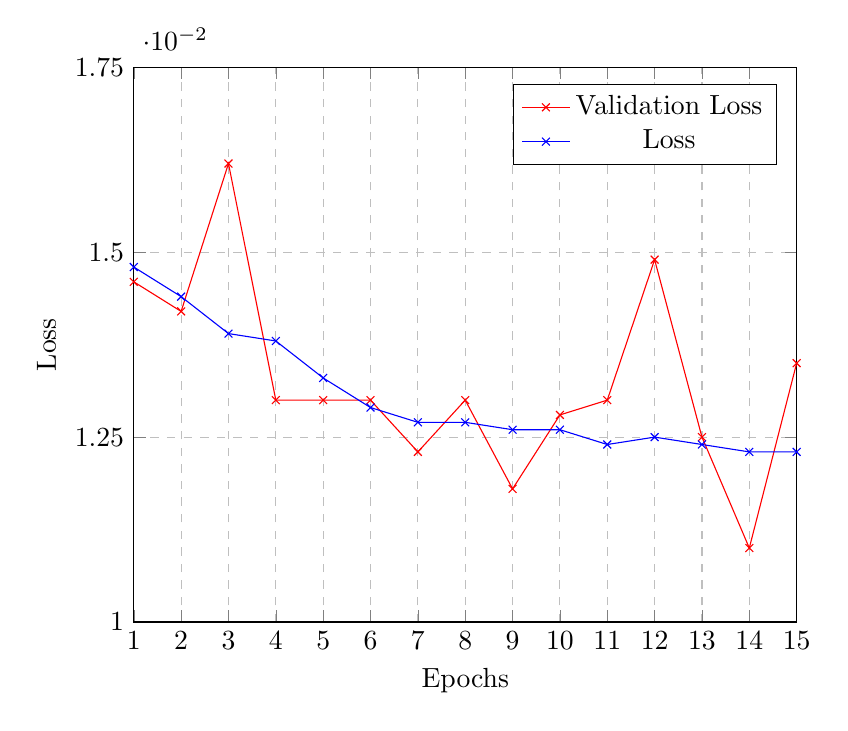
\begin{tikzpicture}
\begin{axis}[
    % title={Courbe de Loss en fonction des epochs},
    xlabel={Epochs},
    ylabel={Loss},
    xmin=1, xmax=15,
    ymin=0.01, ymax=0.0175,
    xtick={0,1,2,3,4,5,6,7,8,9,10,11,12,13,14,15},
    ytick={0.01,0.0125,0.015,0.0175,0.02},
    legend pos=north east,
    ymajorgrids=true,
    xmajorgrids=true,
    grid style=dashed
]

\addplot[
    color=red,
    mark=x,
    ]
    coordinates {
    (1,0.0146)(2,0.0142)(3,0.0162)(4,0.0130)(5,0.0130)(6,0.0130)(7,0.0123)(8,0.0130)(9,0.0118)(10,0.0128)(11,0.0130)(12,0.0149)(13,0.0125)(14,0.0110)(15,0.0135)
    };
    \addlegendentry{Validation Loss}
    
\addplot[
    color=blue,
    mark=x,
    ]
    coordinates {
    (1,0.0148)(2,0.0144)(3,0.0139)(4,0.0138)(5,0.0133)(6,0.0129)(7,0.0127)(8,0.0127)(9,0.0126)(10,0.0126)(11,0.0124)(12,0.0125)(13,0.0124)(14,0.0123)(15,0.0123)
    };
    \addlegendentry{Loss}    
\end{axis}
\end{tikzpicture}
\end{center}
On constate que la loss décroit, ce qui nous confirme que le réseau a bien appris lors de ces epochs. Toutefois ces résultats sont moyennement satisfaisants, car la decroissance de la loss n'est que d'environ $20\%$ et la validation loss ne croit qu'en pics. On peut toutefois observer sur les images que les résultats nous permettent d'identifier du mouvement et la direction globale, mais la position reste assez floue. On constate aussi que quelques erreurs sont générées : sur le premier exemple on observe une tâche jaune non présente dans la groundtruth.
\begin{figure}[h]
    \centering
    \begin{minipage}{0.45\textwidth}
        \centering
        \includegraphics[height=6cm]{Images/FlowNet/flownet_visualization_00001.png}
        %\caption{Première image}
    \end{minipage}
    \hfill
    \begin{minipage}{0.45\textwidth}
        \centering
        \includegraphics[height=6cm]{Images/FlowNet/flownet_visualization_20000.png}
        %\caption{Seconde image}
    \end{minipage}
\end{figure}
\subsection{Estimation de Flot Optique par apprentissage non-supervisé}
\subsubsection{Motivations}
En vue de ce qui a été expliqué précédemment, notamment à propos de la difficulté d'obtenir des images avec le flot optique sans les générer par ordinateur, on s'interrese donc à l'estimation de flot optique par apprentissage non-supervisé, contrairement à ce qui a été fait précédemment.

\subsubsection{Approche technique}
Le principe \cite{basics} pour calculer le flot par apprentissage non-supervisé est de garder l'architecture présentée plus haut du FlowNet Simple, mais d'adapter la loss : 
    \[\mathcal L(u,v,I(x,y,t),I(x,y,t+1))=\ell_{\text{photometric}}(u,v,I(x,y,t),I(x,y,t+1))+\lambda \ell_{\text{smoothness}}(u,v)\]
    Où : \\
    \begin{itemize}
        \item $u,v\in\mathbb R^{H\times W}$  sont les composantes horizontales et verticales du flot prédit.
        \item $\ell_{\text{photometric}}(u,v,I(x,y,t),I(x,y,t+1))=\displaystyle\sum_{i,j}\rho_D(I(i,j,t)-I(i+u_{i,j},j+v_{i,j},t+1))$
        \item $\ell_{\text{smoothness}}(u,v)=\displaystyle\sum_{j}^{H}\sum_{i}^{W}(\rho_S(u_{i,j}-u_{i+1,j}) + \rho_S(u_{i,j}-u_{i,j+1})+\rho_S(v_{i,j}-v_{i+1,j}) + \rho_S(v_{i,j}-v_{i,j+1}))$
        \item $\rho_{S,D}:x\mapsto(x^2+\varepsilon^2)^{\alpha_{S,D}}$ est la fonction de Charbonnier généralisée.
        \item $\lambda$ est un paramètre de régularisation qui décide de l'importance relative pour le flot prédit soit lisse ou non.
    \end{itemize}




\section{Annexes}


% \begin{python}[basicstyle=\ttfamily]
% """ FlowNet model written in TF2/Keras
%     https://arxiv.org/pdf/1504.06852.pdf
% """

% from typing import Dict, Tuple, Optional, Union
% from pathlib import Path
% from copy import deepcopy
% from datetime import datetime

% import numpy as np
% import tensorflow as tf
% from tensorflow.keras import backend as K

% import utils_io as uio
% import utils
% # from utils import visualize_flownet_prediction
% from config import CONFIG_FLOWNET, CONFIG_TRAINING
% import matplotlib.pyplot as plt


% class MalformedNetworkType(Exception):
%     """The provided network type doesn't match one of 'simple' or 'correlation'."""


% class FlowNet:
%     """ FlowNetSimple model from the Computer Vision Group of Freiburg.
%         https://lmb.informatik.uni-freiburg.de/
%         https://lmb.informatik.uni-freiburg.de/Publications/2015/DFIB15/flownet.pdf
%     """

%     def __init__(self, config: Dict):
%         self.config = config

%         self.model = self._construct_network(config)

%     def __getattr__(self, attr):
%         """ Rather than potentially override any of the tf.keras.Model methods by subclassing and defining new methods,
%             create a composition class with self.model:tf.keras.Model and allow attribute calls directly against self.model
%         """
%         return getattr(self.model, attr)

%     @staticmethod
%     def get_simple_model(config: Dict) -> tf.keras.Model:
%         inputs = tf.keras.Input(shape=(384, 512, 6))

%         conv_1 = tf.keras.layers.Conv2D(32, 7, strides=2, padding='same', activation='relu', name='conv1')(inputs)
%         conv_2 = tf.keras.layers.Conv2D(64, 5, strides=2, padding='same', activation='relu', name='conv2')(conv_1)
%         conv_3 = tf.keras.layers.Conv2D(128, 5, strides=2, padding='same', activation='relu', name='conv3')(conv_2)

%         predict_3 = tf.keras.layers.Conv2D(2, 3, strides=1, padding='same', activation=None, name='predict_3')(conv_3)

%         upconv_2 = tf.keras.layers.Conv2DTranspose(64, 4, strides=2, padding='same', activation='relu', name='upconv_2')(conv_3)
%         flow_3 = tf.keras.layers.Conv2DTranspose(2, 4, strides=2, padding='same', activation='relu', name='flow_3')(predict_3)
%         concat_2 = tf.keras.layers.Concatenate(axis=-1, name='concat_2')([upconv_2, conv_2, flow_3])
%         predict_2 = tf.keras.layers.Conv2D(2, 3, strides=1, padding='same', activation=None, name='predict_2')(concat_2)

%         upconv_1 = tf.keras.layers.Conv2DTranspose(32, 4, strides=2, padding='same', activation='relu', name='upconv_1')(concat_2)
%         flow_2 = tf.keras.layers.Conv2DTranspose(2, 4, strides=2, padding='same', activation='relu', name='flow_2')(predict_2)
%         concat_1 = tf.keras.layers.Concatenate(axis=-1, name='concat_1')([upconv_1, conv_1, flow_2])
%         predict_1 = tf.keras.layers.Conv2D(2, 3, strides=1, padding='same', activation=None, name='predict_1')(concat_1)

%         if config['training']:
%             return tf.keras.Model(inputs=inputs, outputs=[predict_3, predict_2, predict_1])

%         return tf.keras.Model(inputs=inputs, outputs=predict_1)


%     def disable_training(self):
%         """Switch model to single-output inference mode"""
%         self.model = tf.keras.Model(
%             inputs=self.model.input,
%             outputs=self.model.output[-1]
%         )

%     def enable_training(self):
%         """ If you need to re-enable training, run this method to have self.model predict the list of 6 predictions
%         """
%         output_layers = [layer.output for layer in self.model.layers if 'predict' in layer.name]
%         self.model = tf.keras.Model(inputs=self.model.layers[0].input, outputs=output_layers)

%     @staticmethod
%     def get_corr_model(config: Dict) -> tf.keras.Model:
%         raise NotImplementedError("The correlation model hasn't been implemented.")

%     @staticmethod
%     def _construct_network(config: Dict) -> tf.keras.Model:
%         if config['architecture'] == 'simple':
%             return FlowNet.get_simple_model(config)
%         if config['architecture'] == 'corr':
%             return FlowNet.get_corr_model(config)

%         raise MalformedNetworkType(f"{config['architecture']}: {MalformedNetworkType.__doc__}")


% class DataGenerator:
%     """ Instantiate then call instance.next_train() to get a generator for training images/labels
%             call instance.next_val() to get a generator for validation images/labels
%     """

%     def __init__(self,
%                  network_type: str,
%                  flo_normalization: Tuple[float, float],
%                  root_path: Path,
%                  batch_size: int,
%                  validation_batch_size: int,
%                  train_ratio: Union[float, int] = 1,
%                  test_ratio: Union[float, int] = 0,
%                  shuffle: bool = False,
%                  augmentations: Optional[Dict] = None):
%         self.network_type = network_type

%         images = list(root_path.glob('*1.ppm'))
%         self.train, self.val, self.test = utils.get_train_val_test(images, train_ratio, test_ratio, shuffle)
%         self.batch_size = batch_size
%         self.validation_batch_size = validation_batch_size
%         self.replace = True
%         self.flo_normalization = flo_normalization
%         self.augmentations = augmentations
        
%     def next_train(self):

%         while True:
%             images = np.random.choice(self.train, self.batch_size, replace=self.replace)
%             img1 = [uio.read(str(img)) for img in images]
%             img2 = [uio.read(str(img).replace('1.ppm', '2.ppm')) for img in images]
%             label = [uio.read(str(img).replace('img1.ppm', 'flow.flo')) for img in images]

%             img1 = utils.normalize_images(img1)
%             img2 = utils.normalize_images(img2)
%             label = utils.normalize_flo(label, self.flo_normalization)

%             if not self.augmentations is None:
%                 img1, img2, label = self._augment(img1, img2, label)

%             if self.network_type == 'simple':
%                 images = np.concatenate([img1, img2], axis=-1)
%             elif self.network_type == 'correlation':
%                 raise NotImplementedError()
%             else:
%                 raise MalformedNetworkType(f'{self.network_type}: {MalformedNetworkType.__doc__}')

%             yield (images, np.array(label))

%     def next_val(self):

%         while True:
%             images = np.random.choice(self.val, self.validation_batch_size, replace=False)
%             img1 = [uio.read(str(img)) for img in images]
%             img2 = [uio.read(str(img).replace('1.ppm', '2.ppm')) for img in images]
%             label = [uio.read(str(img).replace('img1.ppm', 'flow.flo')) for img in images]

%             img1 = utils.normalize_images(img1)
%             img2 = utils.normalize_images(img2)
%             label = utils.normalize_flo(label, self.flo_normalization)

%             if self.network_type == 'simple':
%                 images = np.concatenate([img1, img2], axis=-1)
%             elif self.network_type == 'correlation':
%                 raise NotImplementedError()
%             else:
%                 raise MalformedNetworkType(f'{self.network_type}: {MalformedNetworkType.__doc__}')

%             yield (images, np.array(label))

%     def _augment(self, img1, img2, label):
%         # Augmentations are more awkward because of the Siamese architecture, I can't justify applying different color transforms to each image independently
%         # I'm 100 certain there is a better way to do this as this is extremely inefficient with each call likely containing some portion of each other call.
%         r = np.random.rand(len(self.augmentations))
%         r_inc = 0  # This, with r, are used to randomly turn on/off augmentations so that not every augmentation is applied each time
%         r_onoff = 2/5
%         if 'brightness' in self.augmentations and r[r_inc] <= r_onoff:
%             rdm = np.random.rand(self.batch_size) * self.augmentations['brightness']
%             def brt(x, idx): return tf.image.adjust_brightness(x, rdm[idx])
%             img1 = tf.stack([brt(im, idx) for idx, im in enumerate(img1)], axis=0)
%             img2 = tf.stack([brt(im, idx) for idx, im in enumerate(img2)], axis=0)
%             r_inc += 1
%         if 'multiplicative_colour' in self.augmentations and r[r_inc] <= r_onoff:
%             rdm = np.random.rand(self.batch_size, 3) * (self.augmentations['multiplicative_colour'][1] -
%                                                         self.augmentations['multiplicative_colour'][0]) + self.augmentations['multiplicative_colour'][0]

%             def mc(x, idx): return x * rdm[idx]
%             img1 = tf.clip_by_value(tf.stack([mc(im, idx) for idx, im in enumerate(img1)], axis=0), clip_value_min=0, clip_value_max=1)
%             img2 = tf.clip_by_value(tf.stack([mc(im, idx) for idx, im in enumerate(img2)], axis=0), clip_value_min=0, clip_value_max=1)
%             r_inc += 1
%         if 'gamma' in self.augmentations and r[r_inc] <= r_onoff:
%             rdm = np.random.rand(self.batch_size) * (self.augmentations['gamma'][1] - self.augmentations['gamma'][0]) + self.augmentations['gamma'][0]
%             def gam(x, idx): return tf.image.adjust_gamma(x, gamma=rdm[idx])
%             img1 = tf.stack([gam(im, idx) for idx, im in enumerate(img1)], axis=0)
%             img2 = tf.stack([gam(im, idx) for idx, im in enumerate(img2)], axis=0)
%             r_inc += 1
%         if 'contrast' in self.augmentations and r[r_inc] <= r_onoff:
%             rdm = np.random.rand(self.batch_size) * (self.augmentations['contrast'][1] - self.augmentations['contrast'][0]) + self.augmentations['contrast'][0]
%             def cts(x, idx): return tf.image.adjust_contrast(x, contrast_factor=rdm[idx])
%             img1 = tf.stack([cts(im, idx) for idx, im in enumerate(img1)], axis=0)
%             img2 = tf.stack([cts(im, idx) for idx, im in enumerate(img2)], axis=0)
%             r_inc += 1
%         if 'gaussian_noise' in self.augmentations and r[r_inc] <= r_onoff:
%             rdm = np.random.rand(self.batch_size) * self.augmentations['gaussian_noise']
%             def gau(x, idx): return x + tf.random.normal(x.shape, mean=0.0, stddev=rdm[idx], dtype=x.dtype)
%             img1 = tf.clip_by_value(tf.stack([gau(im, idx) for idx, im in enumerate(img1)], axis=0), clip_value_min=0, clip_value_max=1)
%             img2 = tf.clip_by_value(tf.stack([gau(im, idx) for idx, im in enumerate(img2)], axis=0), clip_value_min=0, clip_value_max=1)
%             r_inc += 1

%         return img1, img2, label


% class EndPointError(tf.keras.losses.Loss):
%     """ EndPointError is the Euclidean distance between the predicted flow vector and the ground truth averaged over all pixels.
%         The resizing is required because the loss is calculated for each flow prediction which occur at different stride levels,
%         resizing effectively averages at that scale.
%     """

%     def call(self, y_true, y_pred):
%         return K.sqrt(K.sum(K.square(tf.image.resize(y_true, y_pred.shape[1:3]) - y_pred), axis=1, keepdims=True))
    




% def show_images(simple_images, label):

%     import matplotlib.pyplot as plt
%     fig, ax = plt.subplots(ncols=2, nrows=2)
%     ax[0, 0].imshow(simple_images[..., :3])
%     ax[0, 1].imshow(simple_images[..., 3:])
%     ax[1, 0].imshow(label[..., 0])
%     ax[1, 1].imshow(label[..., 1])
%     plt.show()

% def visualize_flownet_prediction(flownet, image_id, config, data_path):
%     img1_path = Path(data_path) / f"{image_id}_img1.ppm"
%     img2_path = Path(data_path) / f"{image_id}_img2.ppm"
%     flow_path = Path(data_path) / f"{image_id}_flow.flo"
    
%     # Load images and ground truth flow
%     img1 = uio.read(str(img1_path))
%     img2 = uio.read(str(img2_path))
%     flow_gt = uio.read(str(flow_path))
    
%     # Normalize images for prediction
%     img1_norm = utils.normalize_images([img1])[0]
%     img2_norm = utils.normalize_images([img2])[0]
    
%     # Concatenate images for FlowNet input
%     network_input = np.concatenate([img1_norm, img2_norm], axis=-1)
%     network_input = np.expand_dims(network_input, axis=0)  # Add batch dimension
    
%     # Get prediction
%     flow_pred = flownet.predict(network_input)
    
%     # Handle different output shapes
%     if isinstance(flow_pred, list):
%         flow_pred = flow_pred[-1]  # Get the final prediction if multiple outputs
    
%     # Remove batch dimension if present
%     if len(flow_pred.shape) == 4:
%         flow_pred = flow_pred[0]
    
%     # Debug: print shapes
%     print(f"Flow prediction shape: {flow_pred.shape}")
%     print(f"Ground truth flow shape: {flow_gt.shape}")
    
%     # Denormalize predicted flow
%     # Assuming utils has denormalize_flo function, otherwise use manual method
%     try:
%         flow_pred_denorm = utils.denormalize_flo(flow_pred, config['flo_normalization'])
%     except (AttributeError, NameError):
%         # Manual denormalization
%         flo_min, flo_max = config['flo_normalization']
%         flow_pred_denorm = flow_pred * (flo_max - flo_min) + flo_min
    
%     # Ensure flow_pred_denorm has correct shape (H, W, 2)
%     if len(flow_pred_denorm.shape) == 2:
%         print("Warning: Flow prediction is 2D, reshaping to (H, W, 2)")
%         h, w = flow_pred_denorm.shape
%         flow_pred_denorm = flow_pred_denorm.reshape(h, w, 1)
%         flow_pred_denorm = np.concatenate([flow_pred_denorm, np.zeros_like(flow_pred_denorm)], axis=-1)
    
%     # Resize predicted flow to match ground truth size if needed
%     if flow_pred_denorm.shape[:2] != flow_gt.shape[:2]:
%         print(f"Resizing flow from {flow_pred_denorm.shape[:2]} to {flow_gt.shape[:2]}")
%         import cv2
%         flow_pred_denorm = cv2.resize(flow_pred_denorm, 
%                                       (flow_gt.shape[1], flow_gt.shape[0]), 
%                                       interpolation=cv2.INTER_LINEAR)
    
%     # Create visualization with white background
%     fig, axes = plt.subplots(2, 2, figsize=(12, 10), facecolor='white')
%     fig.patch.set_facecolor('white')
    
%     # Row 1: Input images
%     axes[0, 0].imshow(img1.astype(np.uint8))
%     axes[0, 0].set_title('Image 1', fontsize=14, fontweight='bold')
%     axes[0, 0].axis('off')
    
%     axes[0, 1].imshow(img2.astype(np.uint8))
%     axes[0, 1].set_title('Image 2', fontsize=14, fontweight='bold')
%     axes[0, 1].axis('off')
    
%     # Row 2: Ground truth flow and predicted flow
%     # Ground truth flow visualization
%     flow_gt_vis = flow_to_color(flow_gt)
%     axes[1, 0].imshow(flow_gt_vis)
%     axes[1, 0].set_title('Flot GroundTruth ', fontsize=14, fontweight='bold')
%     axes[1, 0].axis('off')
    
%     # Predicted flow visualization
%     flow_pred_vis = flow_to_color(flow_pred_denorm)
%     axes[1, 1].imshow(flow_pred_vis)
    
%     # Calculate EPE for title
%     flow_error = np.sqrt(np.sum((flow_gt - flow_pred_denorm)**2, axis=-1))
%     axes[1, 1].set_title(f'Flot Prédit', fontsize=14, fontweight='bold') #(EPE: {flow_error.mean():.2f})
%     axes[1, 1].axis('off')
    
%     plt.tight_layout()
%     plt.savefig(f'flownet_visualization_{image_id}.png', dpi=150, bbox_inches='tight', facecolor='white')
%     plt.show()
    
%     # Print statistics
%     print(f"\n=== FlowNet Visualization Statistics ===")
%     print(f"Image ID: {image_id}")
%     print(f"Image shape: {img1.shape}")
%     print(f"Flow shape: {flow_gt.shape}")
%     print(f"Ground truth flow range: [{flow_gt.min():.2f}, {flow_gt.max():.2f}]")
%     print(f"Predicted flow range: [{flow_pred_denorm.min():.2f}, {flow_pred_denorm.max():.2f}]")
%     print(f"Average EPE (End-Point Error): {flow_error.mean():.3f}")
%     print(f"Max EPE: {flow_error.max():.3f}")


% def flow_to_color(flow, max_flow=None):
%     """
%     Convert optical flow to RGB color representation using Middlebury color scheme.
    
%     Args:
%         flow: Flow field (H, W, 2) with (u, v) components
%         max_flow: Maximum flow magnitude for normalization. If None, uses max from flow.
    
%     Returns:
%         RGB image (H, W, 3) representing the flow
%     """
%     # Handle edge cases
%     if flow is None:
%         raise ValueError("Flow is None")
    
%     # Ensure flow has correct shape
%     if len(flow.shape) == 2:
%         # If 2D, assume it's a single channel and create dummy second channel
%         flow = np.stack([flow, np.zeros_like(flow)], axis=-1)
    
%     if len(flow.shape) != 3 or flow.shape[2] != 2:
%         raise ValueError(f"Flow must have shape (H, W, 2), got {flow.shape}")
    
%     u = flow[:, :, 0]
%     v = flow[:, :, 1]
    
%     # Calculate flow magnitude and angle
%     mag = np.sqrt(u**2 + v**2)
%     angle = np.arctan2(-v, -u) / np.pi
    
%     # Normalize magnitude
%     if max_flow is None:
%         max_flow = np.max(mag)
    
%     if max_flow > 0:
%         mag = mag / max_flow
    
%     # Create Middlebury color wheel
%     fk = (angle + 1) / 2 * (ncols - 1)  # -1~1 mapped to 0~ncols-1
%     k0 = np.floor(fk).astype(np.int32)
%     k1 = k0 + 1
%     k1[k1 == ncols] = 0
%     f = fk - k0
    
%     ncolors = colorwheel.shape[0]
    
%     img = np.zeros((flow.shape[0], flow.shape[1], 3), dtype=np.float32)
    
%     for i in range(3):
%         tmp = colorwheel[:, i]
%         col0 = tmp[k0] / 255.0
%         col1 = tmp[k1] / 255.0
%         col = (1 - f) * col0 + f * col1
        
%         # Increase saturation with magnitude
%         idx = mag <= 1
%         col[idx] = 1 - mag[idx] * (1 - col[idx])
%         col[~idx] = col[~idx] * 0.75  # Out of range
        
%         img[:, :, i] = col
    
%     return img


% def make_colorwheel():
%     """
%     Generate color wheel according to Middlebury color code
%     for optical flow visualization.
    
%     Returns:
%         colorwheel: Color wheel with shape (ncols, 3)
%     """
%     # Relative lengths of color transitions
%     RY = 15
%     YG = 6
%     GC = 4
%     CB = 11
%     BM = 13
%     MR = 6
    
%     ncols = RY + YG + GC + CB + BM + MR
%     colorwheel = np.zeros((ncols, 3), dtype=np.uint8)
    
%     col = 0
    
%     # RY
%     colorwheel[col:col+RY, 0] = 255
%     colorwheel[col:col+RY, 1] = np.floor(255 * np.arange(RY) / RY)
%     col += RY
    
%     # YG
%     colorwheel[col:col+YG, 0] = 255 - np.floor(255 * np.arange(YG) / YG)
%     colorwheel[col:col+YG, 1] = 255
%     col += YG
    
%     # GC
%     colorwheel[col:col+GC, 1] = 255
%     colorwheel[col:col+GC, 2] = np.floor(255 * np.arange(GC) / GC)
%     col += GC
    
%     # CB
%     colorwheel[col:col+CB, 1] = 255 - np.floor(255 * np.arange(CB) / CB)
%     colorwheel[col:col+CB, 2] = 255
%     col += CB
    
%     # BM
%     colorwheel[col:col+BM, 2] = 255
%     colorwheel[col:col+BM, 0] = np.floor(255 * np.arange(BM) / BM)
%     col += BM
    
%     # MR
%     colorwheel[col:col+MR, 2] = 255 - np.floor(255 * np.arange(MR) / MR)
%     colorwheel[col:col+MR, 0] = 255
    
%     return colorwheel


% # Generate the Middlebury color wheel
% colorwheel = make_colorwheel()
% ncols = colorwheel.shape[0]


% def visualize_multiple_samples(flownet, image_ids, config, data_path):
%     """
%     Visualize multiple samples in a grid.
    
%     Args:
%         flownet: Trained FlowNet model
%         image_ids: List of image identifiers
%         config: Configuration dictionary
%         data_path: Path to the dataset directory
%     """
%     n_samples = len(image_ids)
%     fig, axes = plt.subplots(n_samples, 4, figsize=(16, 4*n_samples))
    
%     if n_samples == 1:
%         axes = axes.reshape(1, -1)
    
%     for idx, image_id in enumerate(image_ids):
%         # Load data
%         img1_path = Path(data_path) / f"{image_id}_img1.ppm"
%         img2_path = Path(data_path) / f"{image_id}_img2.ppm"
%         flow_path = Path(data_path) / f"{image_id}_flow.flo"
        
%         img1 = uio.read(str(img1_path))
%         img2 = uio.read(str(img2_path))
%         flow_gt = uio.read(str(flow_path))
        
%         # Get prediction
%         flow_pred = flownet.predict(network_input, verbose=0)
        
%         # Handle different output shapes
%         if isinstance(flow_pred, list):
%             flow_pred = flow_pred[-1]
        
%         # Remove batch dimension if present
%         if len(flow_pred.shape) == 4:
%             flow_pred = flow_pred[0]
        
%         # Denormalize
%         try:
%             flow_pred_denorm = utils.denormalize_flo(flow_pred, config['flo_normalization'])
%         except (AttributeError, NameError):
%             flo_min, flo_max = config['flo_normalization']
%             flow_pred_denorm = flow_pred * (flo_max - flo_min) + flo_min
        
%         # Ensure correct shape and size
%         if len(flow_pred_denorm.shape) == 2:
%             h, w = flow_pred_denorm.shape
%             flow_pred_denorm = flow_pred_denorm.reshape(h, w, 1)
%             flow_pred_denorm = np.concatenate([flow_pred_denorm, np.zeros_like(flow_pred_denorm)], axis=-1)
        
%         if flow_pred_denorm.shape[:2] != flow_gt.shape[:2]:
%             import cv2
%             flow_pred_denorm = cv2.resize(flow_pred_denorm, 
%                                           (flow_gt.shape[1], flow_gt.shape[0]), 
%                                           interpolation=cv2.INTER_LINEAR)
        
%         # Visualize
%         axes[idx, 0].imshow(img1.astype(np.uint8))
%         axes[idx, 0].set_title(f'{image_id} - Image 1')
%         axes[idx, 0].axis('off')
        
%         axes[idx, 1].imshow(img2.astype(np.uint8))
%         axes[idx, 1].set_title(f'{image_id} - Image 2')
%         axes[idx, 1].axis('off')
        
%         axes[idx, 2].imshow(flow_to_color(flow_gt))
%         axes[idx, 2].set_title('Ground Truth')
%         axes[idx, 2].axis('off')
        
%         axes[idx, 3].imshow(flow_to_color(flow_pred_denorm))
%         epe = np.sqrt(np.sum((flow_gt - flow_pred_denorm)**2, axis=-1)).mean()
%         axes[idx, 3].set_title(f'Prediction (EPE: {epe:.2f})')
%         axes[idx, 3].axis('off')
    
%     plt.tight_layout()
%     plt.savefig('flownet_multiple_samples.png', dpi=150, bbox_inches='tight')
%     plt.show()
% def main():
%     config_network = deepcopy(CONFIG_FLOWNET)
%     config_training = deepcopy(CONFIG_TRAINING)
    
%     flownet = FlowNet(config_network)
%     flownet.load_weights("/Users/oscar/Etudes/Ecole/PR/FlowNet_v1_TF2-master/src/flow.weights.h5")
    
%     # IMPORTANT: switch to inference mode (single output)
%     flownet.disable_training()
    
%     # Visualize a single sample with detailed view
%     visualize_flownet_prediction(
%         flownet=flownet,
%         image_id="00001",  # Change this to any image ID
%         config=config_network,
%         data_path=config_training['img_path']
%     )
    
%     # Optional: Visualize multiple samples in a grid
%     # visualize_multiple_samples(
%     #     flownet=flownet,
%     #     image_ids=["00001", "00002", "00003"],
%     #     config=config_network,
%     #     data_path=config_training['img_path']
%     # )

% if __name__ == "__main__":
%     main()
% \end{python}

\printbibliography[heading=bibintoc,title={Références}]
\end{document}

